\documentclass[10pt]{article}
\usepackage{../../local}
\usepackage{mathrsfs}
\urlstyle{same}

\newcommand{\classcode}{EE 120}
\newcommand{\classname}{Signals and Systems}
\renewcommand{\maketitle}{%
\hrule height4pt
\large{Eric Du \hfill \classcode}
\newline
\large{HW 02} \Large{\hfill \classname \hfill} \large{\today}
\hrule height4pt \vskip .7em
\small{Header styling inspired by CS 70: \url{https://www.eecs70.org/}}
\normalsize
}
\linespread{1.1}
\begin{document}
	\maketitle
	\section*{Collaborators} 
	I worked with the following people to complete this homework:
	\begin{itemize}
		\item Teja Nivarthi: 3036508567
		\item Nikhil Maserang: 3036978230
		\item Sanjit Shirol: 3037699966
		\item Ralph Cao: 3037721429
	\end{itemize}
	\pagebreak
	\section*{Problem 1}
	Determine whether or not each of the followoing continuous-time or discrete-time signals is periodic. If the signal
	is periodic, determine its fundamental period.
	\begin{enumerate}[label=\alph*)]
		\item \( x(t) = 3 \cos(4t + \frac{\pi}{3}) \) 

			\begin{solution}
				This is a cosine signal, so it is periodic. The fundamental period is 
				\( \frac{2\pi}{4} = \frac{\pi}{2}\)  
			\end{solution}
		\item \( x(t) = e^{i(\pi t - 1)} \) 

			\begin{solution}
				Express \( e^{i(\pi t - 1)} = \cos(\pi t - 1) + i \sin(\pi t - 1) \). Both parts are periodic, 
				with a period of 2. 
			\end{solution}
		\item \( x(t) = \sum_{n = -\infty}^{\infty} e^{-(2t - n)}u(2t -n) \) 

			\begin{solution}
				For integer values of \( 2t \), the summation is the same, except shifted by a constant amount because 
				the value of \( n \) where the step function \( u(t) \) is 1 changes. This doesn't change the value of 
				the infinite sum however, becuase our summation over \( n \) goes from \( -\infty \) to 
				\( \infty \) so we can just shift by whatever \( 2t \) was to recover the same sum. 

				For non-integral values of \( 2t \), the summation over \( n \) doesn't change, but the value 
				of \( e^{-(2t - n)} \) changes. This repeats at every integer (because of the earlier argument), so 
				therefore the summation will repeat at every integer. This means that this signal is periodic 
				when \( 2t \) is an integer, or in other words it has a half-integer period: \( \frac{1}{2} \).   
			\end{solution}
		\item \( x[n] = \sin[\frac{n}{8} - \pi] \)

			\begin{solution}
				For \( n = \{1, 2, \dots, 7\} \), the argument to the sine function is different, but every \( 8 \) 
				inputs the cycle repeats, so therefore the fundamental period is 8.
			\end{solution}
	\end{enumerate}
	\pagebreak
	\section*{Problem 2}
	For each of the following systems defined by their LCCDE, specify the system is i) linear or not, 
	ii) time-invariant or not, iii) memoryless or not, iv) causal or not, and v) BIBO stable or not. Show 
	your work along with your conclusions to get credit. For all the sub-questions, \( x(t) \) or 
	\( x[n] \) is the input, and \( y(t)  \) or  \( y[n] \) is the system output.
	\begin{enumerate}[label=\alph*)]
		\item \( y(t) = x(t - 2) + x(2 - t) \) 

			\begin{solution}
				\begin{itemize}
					\item Linear, because given two signasl \( x_1(t) \) and \( x_2(t) \), define a new signal 
						\( x'(t) = ax_1(t) + bx_2(t) \), then \( y'(t) \) is
						\[
						y'(t) = ax_1(t - 2) + bx_2(t - 2) + ax_1(2 - t) + bx_2(2 - t) = ay_1(t) + by_2(t)
						\] 
						another argument for this is that given a signal \( x(t) = 0 \) we get an output
						\( y(t) = 0 \), so it satisfes the zero-input zero-output property. 
					\item Not time invariant, because given a signal \( x'(t) = x(t - T) \), the output is: 
						\[
						y'(t) = x'(t - 2) + x'(2 - t) = x(t - 2 - T) + x(2 - t - T) 
						\] 
						But \( y(t - T) = x(t - 2 - T) + x(2 - t + T) \); they're not equal, so the system is not
						 time invariant.
					\item This is not memoryless, because the output at time \( t \), requires knowledge of 
						\( x(t - 2) \). 
					\item It's not causal, because \( t = 0 \), then the system \( y(t) \) depends on the 
						 \( x(2) \), implying it's not causal.
					\item This system is BIBO stable, because for a bounded input \( x(t) \), the output 
						\( y(t) \) takes in two bounded values, hence the output must be bounded. 
				\end{itemize}
			\end{solution}
		\item \( y[n] = \sum_{k = 0}^{4}(-1)^{k}x[n - k] \)

			\begin{solution}
				\begin{itemize}
					\item Linear, because all sums by themselves are linear and the terms within the summation 
						are also linear. Also, zero input give zero output.
					\item Time invariant, because given a signal \( x'[n] = x[n - m] \), the output \( y[n] \) is:
						\[
							y[n] = \sum_{k = 0}^{4}(-1)^{k}x'[n - k] = \sum_{k =0}^{4}(-1)^{k}x[n - m - k]
						\] 
						Then, \( y[n - m] \) is given by: 
						\[
							y[n - m] = \sum_{k = 0}^{4}(-1)^{k}x[n - m - k]	
						\] 
						They match, as desired. 
					\item The system is not memoryless, because the output \( y[n] \) depends on previous 
						values \( x[n - 1] \) thorugh \( x[n - 4] \). 
					\item The system is causal, because it doesn't depend on future values of \( n \).  
					\item This system is BIBO stable, because given a bounded \( x[n] \), the output 
						\( y[n] \) sums over four bounded values, which gives us a resulting bounded output.
				\end{itemize}
			\end{solution}
		\item \( y[n] = \cos[x[n] + \frac{\pi}{3}] \) 

			\begin{solution}
				\begin{itemize}
					\item Linear: Given a zero input, \( y[n] = \cos[\pi / 3] \neq 0 \). 
					\item Time invariant: Given an input signal \( x'[n] = x[n - n_0] \), the signal output 
						is: 
						\[
							y'[n] = \cos\left[x'[n] + \frac{\pi}{3}\right] = 
							\cos\left[x[n - n_0] + \frac{\pi}{3}\right] = y[n - n_0]
						\] 
						so the signal is delayed by a constant \( n_0 \), hence it is time invariant. 
					\item Memoryless: The system only depends on \( n \). 
					\item Causal: memoryless implies causal.
					\item The system is BIBO stable, because given a bounded \( x[n] \), \( \cos[x[n] + \pi /3] \) 
						returns a bounded value.
				\end{itemize}
			\end{solution}
		\item \( y(t) = x(t) v(t) \), where \( v(t)  \) is a fixed signal such that 
			\begin{itemize}
				\item  For all \( t <0 \), \( v(t) = 0 \) 
				\item For every \( B \in \R \), there exists \( T \in \R \) such that \( v(T) > B \)
			\end{itemize}

			\begin{solution}
				\begin{itemize}
					\item Linear: Given a zero input, the output is always zero.
					\item Not time invariant: Given an input signal \( x'(t) = x(t - t_0) \), the output is given by: 
						\[
						y'(t) = x'(t)v(t) = x(t - t_0) v(t)  \neq y(t - t_0)
						\] 
					\item Memoryless: the signal only depends on \( t \). 
					\item Causal: memoryless implies causality.
					\item The system is not BIBO stable, becuase given a bounded input \( x(t) \), there are 
						signals \( v(t) \) (e.g. a signal that is always infinite) which could return 
						an unbounded value for \( y(t) \).  

						Alternatively, one could argue that given a bounded input \( x(t) = 1 \), then 
						\( y(t) = v(t) \), but \( v(t)  \) is necessarily unbounded (by its description), so the 
						output signal is necessarily unbounded. 
				\end{itemize}
			\end{solution}
	\end{enumerate}
	\pagebreak
	\section*{Problem 3}
	The causal, discrete time LTI filter \( \mathcal F \) is shown below,
	\begin{center}
		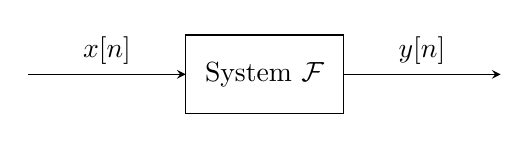
\begin{tikzpicture}
			\draw[-stealth] (-3, 0) -- node[midway, above] {\( x[n] \) } (-1, 0);
			\draw (-1, -0.5) rectangle (1, 0.5);
			\node at (0, 0) {System \( \mathcal F\) };
			\draw[-stealth](1, 0) -- node[midway, above] {\( y[n] \) } (3, 0) ;
		\end{tikzpicture}
	\end{center}
	is characterized by the recursive difference equation \( y[n] = \alpha y[n - N] + x[n] \), where 
	\( |\alpha| < 1 \) and \( N \in \{1, 2, 3, \dots\}  \). Assume systems start at rest, that is for \( n < 0 \), 
	\( x[n], y[n] = 0 \). 
	\begin{enumerate}[label=\alph*)]
		\item Draw the block diagram of this system for \( N = 2 \). 
			
			\begin{solution}
				For \( N = 2 \), the block diagram is: 
				\begin{center}
					\begin{tikzpicture}[scale=1.5]
						\node (A) at (-0.5, 0) {+};
						\draw[-stealth] (-3, 0) -- node[midway, above] {\( x[n] \) } (-.8, 0);
						\draw (A) circle (0.3);
						\draw (-0.2, 0) -- (1, 0);
						\filldraw (1, 0) circle (0.05);
						\draw[-stealth] (1, 0) -- (1, -1);
						\draw (0.75, -1.5) rectangle node {\( \mathcal D \)} (1.25, -1);
						\draw[-stealth] (0.75, -1.25) -- (-0.25, -1.25);
						\draw (-0.75, -1.5) rectangle node {\( \mathcal D \) }(-0.25, -1);
						\draw[-stealth]	(1, 0) -- node[midway, above] {\( y[n] \) } (3, 0) ;
						\draw[-stealth] (-0.5, -1) -- node[midway, left] {\( \alpha \) } (-0.5, -0.3);
					\end{tikzpicture}
				\end{center}
			\end{solution}
		\item Determine an expression for \( f[n] \), where \( f \) is the impulse response of the filter. Express
			your answer in terms of \( \alpha \) and \( N \). 
			\begin{solution}
				The system is definde as:
				\[
					y[n] = \alpha y[n - N] + x[n]
				\] 
				Expanding this out further:
				\[
					y[n] = \alpha(y[n - N] + x[n - N]) + x[n] = \alpha(\alpha (y[n -2N] + x[n - 2N]) + x[n - N]) + 
					x[n]
				\] 
				Therefore, in general:
				\[
					y[n] = \sum_{k = 0}^{\left\lfloor n/N \right\rfloor} \alpha^{k} x[n - kN]
				\] 
				Now, plugging in \( x[n] = \delta[n] \), then we have:
				\[
					f[n] = \sum_{k = 0}^{n / N}\alpha ^{k}\delta[n - kN]
				\] 
			\end{solution}
		\item Provide well-labeled sketches of \( f[n] \) for 
			\begin{enumerate}[label=\roman*)]
				\item \( \alpha = \frac{1}{2} \) and \( N = 2 \) 
				\item \( \alpha = \frac{1}{\sqrt{2} } \) and \( N = 2 \). 
				\item \( \alpha = \frac{1}{2} \) and \( N = 4 \)
			\end{enumerate}
			Describe, in simple terms, the respective effects of \( \alpha \) and \( N \) on the qualitative features 
			of the impulse response \( f \). 

			\begin{solution}
				I give up on drawing this in \LaTeX{}, here's the plots I drew on my ipad:
				\begin{enumerate}[label=\roman*)]
					\item 
						\begin{center}
							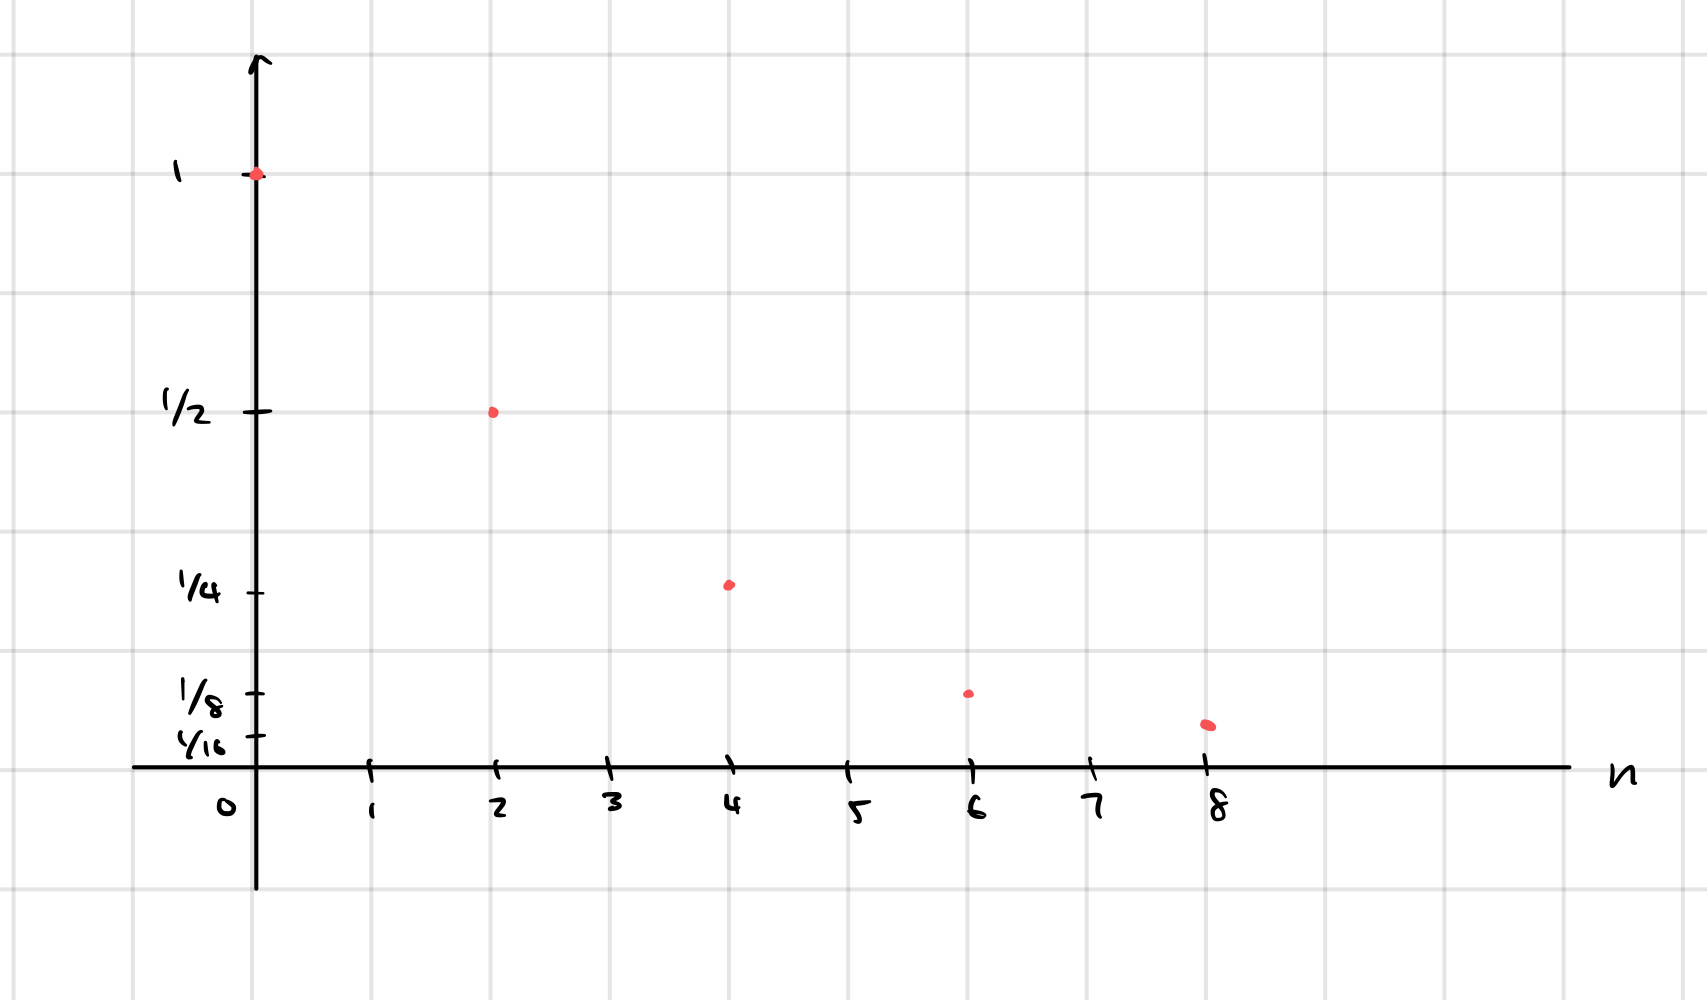
\includegraphics[scale=0.2]{q3ci.jpeg}
						\end{center}
					\item 
						\begin{center}
							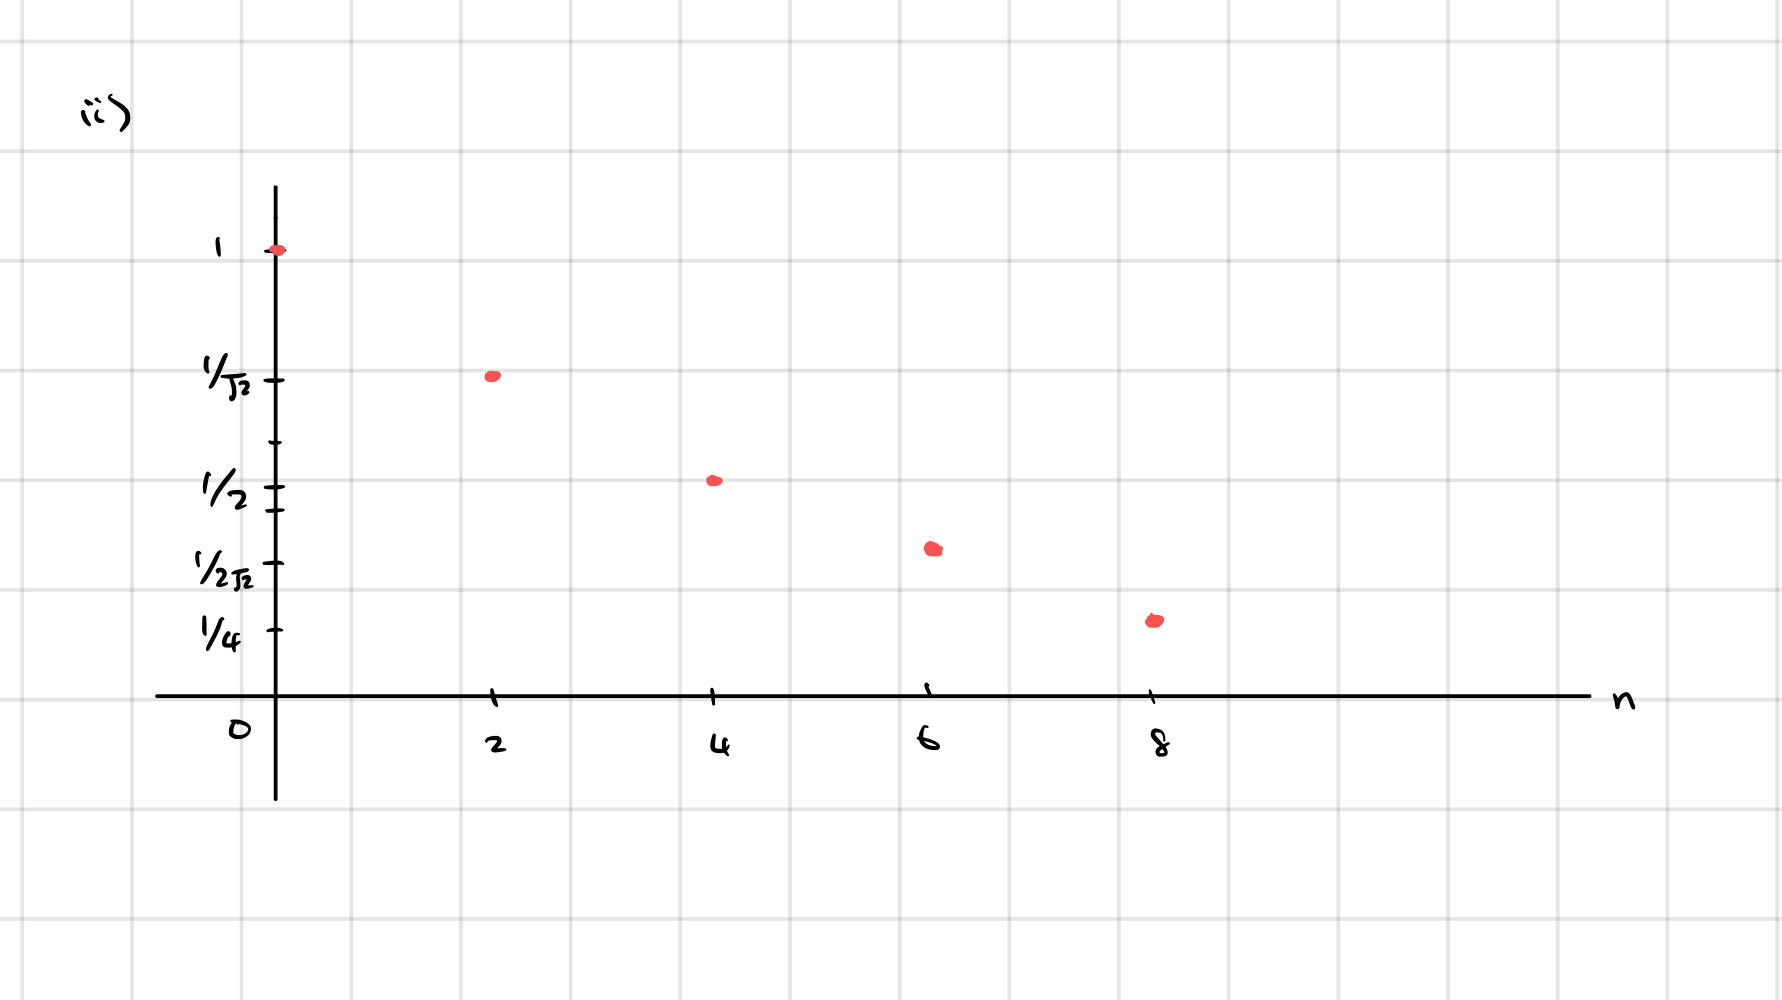
\includegraphics[scale=0.2]{q3cii.jpeg}
						\end{center}
					\item 
						\begin{center}
							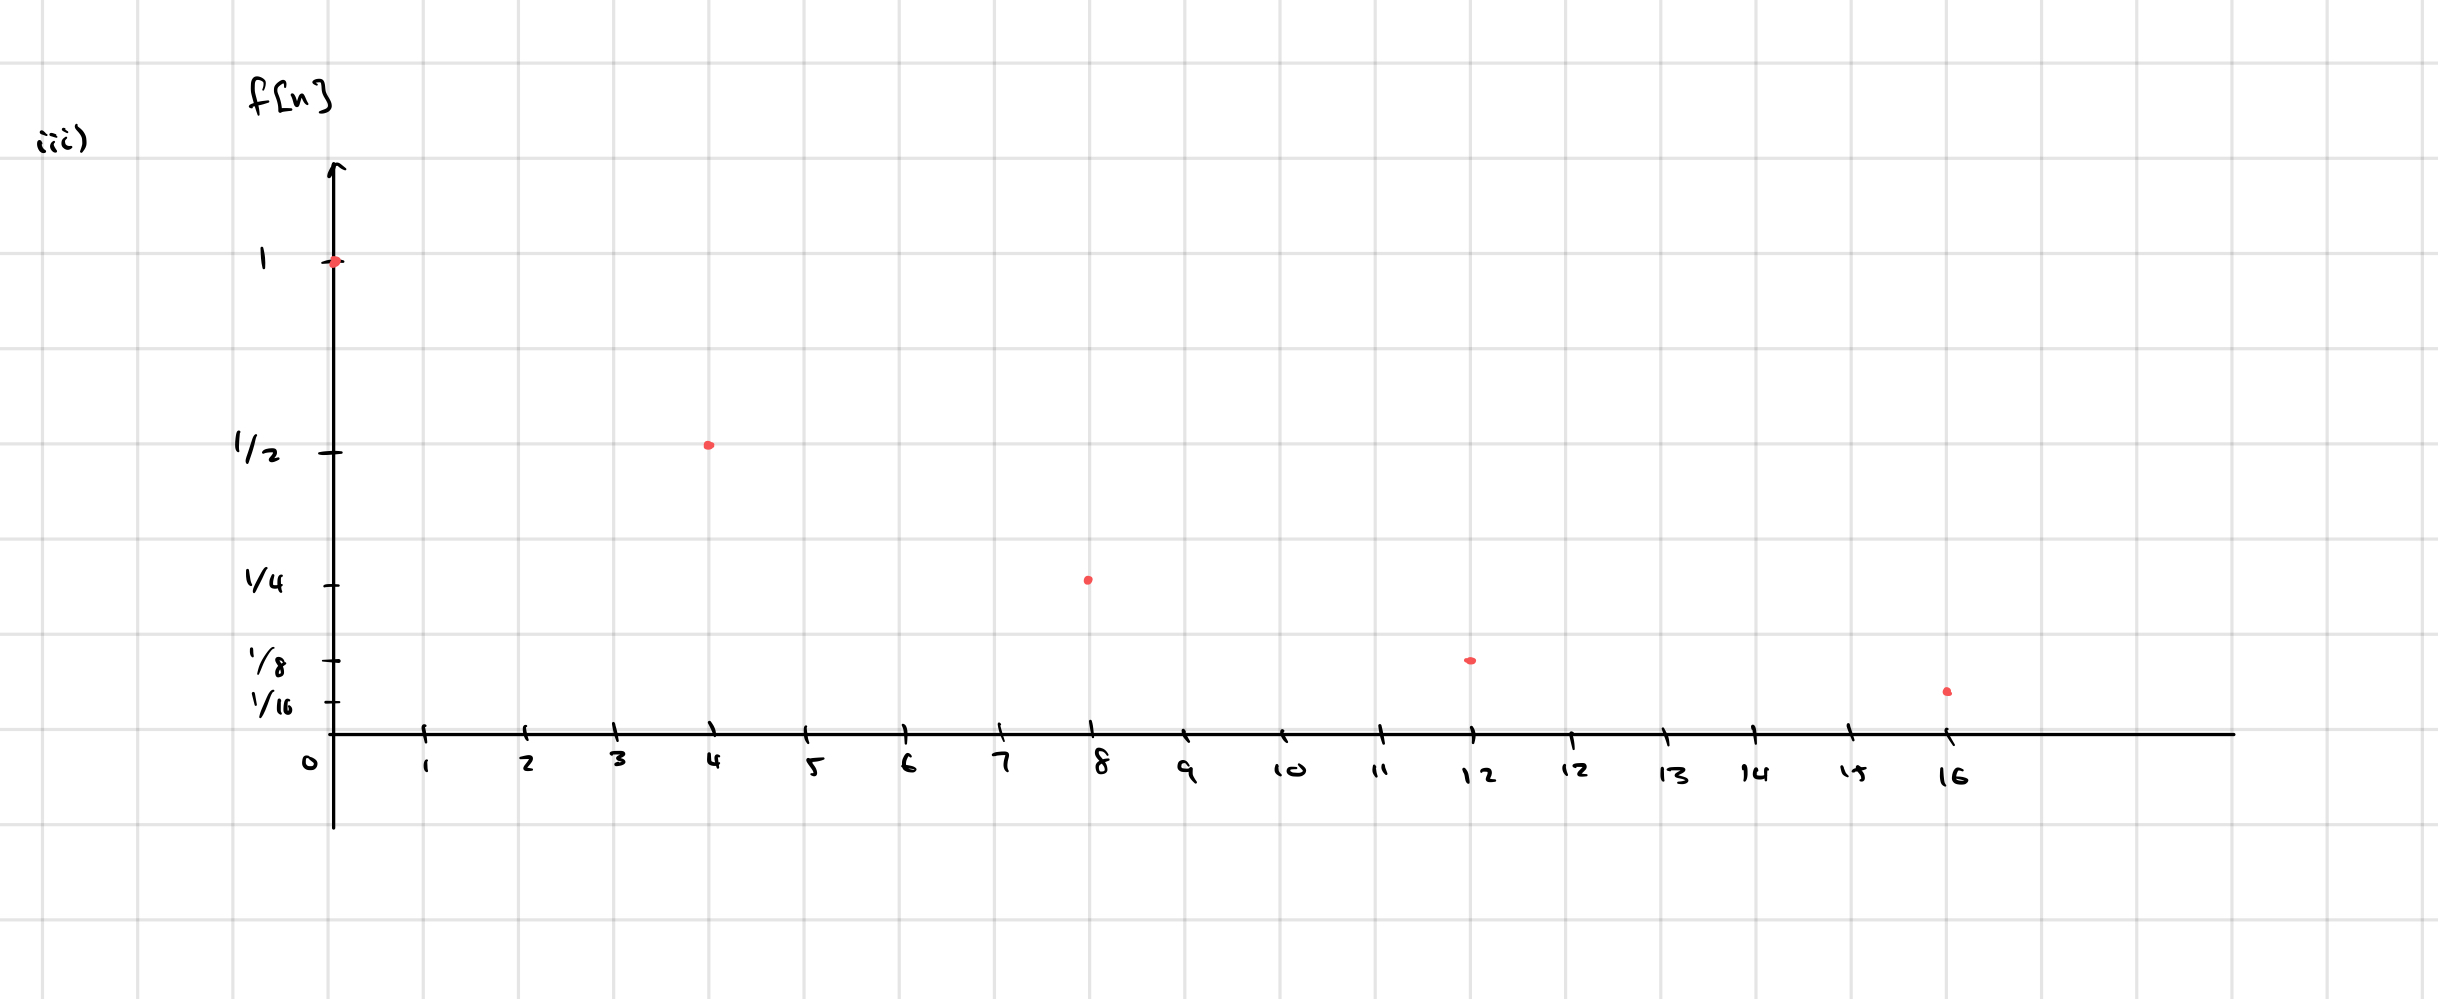
\includegraphics[scale=0.15]{q3ciii.jpeg}
						\end{center}
				\end{enumerate}
			\end{solution}
	\end{enumerate}
	\pagebreak
	\section*{Problem 4}
	For the following system with \( x(t) = e^{-t}u(t) \) as input, \( y(t)  \) as output
	\[
		\dv{y}{t} + \frac{1}{3}y(t) = x(t)
	\] 
	Assume the system is at rest.
	\begin{enumerate}[label=\alph*)]
		\item Determine the homogeneous solution to the output of this system. \\
			\textit{Hint:} Assume the solution is of the form \( Ae^{st} \) where \( A \neq 0 \). 

			\begin{solution}
				The homogeneous solution is when \( x(t) = 0 \). 
				We use the Ansatz of \(y =  Ae^{st} \), so \( \dv{y}{t} = Ase^{st} \):
				\[
					Ase^{st} + \frac{A}{3}e^{st} = 0 \implies s + \frac{1}{3} = 0 \implies s = -\frac{1}{3}
				\] 
				so the homogeneous solution is \( Ae^{-t / 3} \).
			\end{solution}
		\item Determine the particular solution to the output of this system\\
			\textit{Hint:} Assume the solution is of the form \( Ke^{bt}u(t)  \) where \( K \neq 0 \)

			\begin{solution}
				Here, we're trying to solve the differential equation 
				\[
					\dv{y}{t} + \frac{1}{3}y(t) = e^{-t}u(t)
				\] 
				For \( t < 0 \), the right hand side is 0, so we have \( y(t) = 0 \) for \( t < 0 \). For \( t \ge 0 \), 
				\( u(t) = 1 \), so our Ansatz is \( Ke^{bt} \), and we have:
				\[
					\dv{y}{t} + \frac{1}{3}y(t) = e^{-t}
				\] 
				Therefore: 
				\[
				Kbe^{bt} +\frac{1}{3}Ke^{bt} = e^{-t} \implies Ke^{bt}\left(b + \frac{1}{3}\right) = e^{-t}
				\] 
				Now, we match the exponents: we want the exponent to be \( e^{-t} \), implying that \( b = -1 \). 
				Then, we have:
				\[
				K\left( -1 + \frac{1}{3} \right) = 1\implies K = -\frac{3}{2}
				\]  
			\end{solution}
		\item Determine the output of this system, when \( x(t) = e^{-t}u(t) \) is the input. 
			
			\begin{solution}
				The output of the system is going to be a superposition of the homogeneous and particular solution, 
				so:
				\[
				y(t) = Ae^{-t / 3} - \frac{3}{2}e^{-t}u(t)
				\] 
				The condition of the system being at rest is the condition that \( y(0) = 0 \), implying that 
				\[
				A - \frac{3}{2} = 0 \implies A = \frac{3}{2}
				\] 
				Therefore: 
				\[
				y(t) = \frac{3}{2}\left( e^{-t / 3} - e^{-t}u(t) \right) 
				\] 
			\end{solution}
		\item Now let the input be \( \hat{x} = x(t - T) = e^{-(t - T)}u(t - T) \), determine the input 
			\( \hat{y}(t) \) of this system. Show that \( \hat{y}(t) = y(t- T) \). 

			\begin{solution}
				All we need to do is show that the system is time invariant. Given a signal \( \hat{x} = 
				x(t - T)\), then the differential equation looks like:
				\[
					\dv{\hat{y}}{t} + \frac{1}{3}\hat{y}(t) = \hat{x}(t) = x(t - T)
				\] 
				And since the differential equation has the same form (i.e. we can substitute 
				\( t' = t - T \) and we get the exact same DE, then this implies that 
				\( \hat{y}(t) = y(t - T) \).
			\end{solution}
	\end{enumerate}
	\pagebreak
	\section*{Problem 5}
	Consider the following system according to its diagram. Assume the system is initially at rest, that is for 
	\( n < 0 \), \( x[n], y[n] = 0 \). 
	\begin{center}
		\begin{tikzpicture}[scale=1.5]
			\node (r) at (0, 0) {\( r[n] \) };
			\draw[-stealth] (-3, 0) -- node[midway, above] {\( x[n] \) } (-2, 0);
			\draw (-1.7, 0) circle (0.3) node {+}; 
			\draw[-stealth] (-1.4, 0) -- (r);
			\draw[-stealth] (r) -- (1.4, 0);
			\draw(1.7, 0) circle (0.3) node {+};
			\draw[-stealth] (2, 0) -- node[midway, above] {\( y[n] \) } (3, 0);
			\draw [-stealth] (r) -- (0, -1);
			\draw (-0.5, -2) rectangle node {\( \mathcal D \)}(0.5, -1) ;
			\draw[-stealth] (0.5, -1.5) -- node[midway, above] {1} (1.7, -1.5) -- (1.7, -0.3);
			\draw[-stealth] (-0.5, -1.5) -- node[midway, above] {-2} (-1.7, -1.5) -- (-1.7, -0.3);
		\end{tikzpicture}
	\end{center}
	\begin{enumerate}[label=\alph*)]
		\item Express the output \( y[n] \) with respect to \( x[n]  \) with a recursive equation. 

			\begin{solution}
				We can express \( r[n] \) as:
				\[
					r[n] = x[n] - 2r[n - 1]
				\] 
				then, we can express \( y[n] \) as:
				\[
					y[n] = r[n] + r[n - 1]
				\] 
				This implies:
				\[
					y[n] = x[n] - 2r[n - 1] + r[n - 1] = x[n] - r[n - 1] = x[n] - x[n - 1] + 2(x[n - 2] - 2r[n -3])
				\] 
				So this simplifies to:
				\[
					y[n] = x[n] + \sum_{k = 0}^{n}(-2)^{k}x[n - k - 1]
				\] 
				The summation stps at \( n \) becuase for \( n < 0 \), \( x[n] = 0 \). 
			\end{solution}
		\item For \( x[n] = \delta[n] \), find \( r[n] \) for all \( n \). 

			\begin{solution}
				For \( x[n] = \delta[n] \), then we have  \( r[n] = \delta[n] - 2r[n-1] = \delta[n] - 2(\delta[n-1]
				- 2r[n - 2])\). Writing this out as a summation, we have:
				\[
					r[n] = \sum_{k = 0}^{n} (-2)^{k}\delta[n - k]
				\] 
				So for positive \( n > 0 \), only \( k = n \) matters, since that's the only term that makes 
				\( \delta[n - k] \) nonzero. 
				For \( n < 0 \), the system should always be 0, so therefore we have: 
				\[
					r[n] = (-2)^{n}u[n]
				\] 
			\end{solution}
		\item Find this system's impulse response. 

			\begin{solution}
				The impulse response is given by:
				\[
					y[n] = \delta[n] + \sum_{k = 0}^{n}(-2)^{k}\delta[n - k - 1] 
				\] 
				For \( n \ge 0 \), we have \( y[n] = 1 \) for \( n = 0 \), then for other values of \( y[n] \) we
				have:
				\[
					y[n] = (-2)^{n - 1}u[n]
				\] 
				The exponent of \( n - 1 \) is here becuase within the summation only \( k = n - 1 \) matters, 
				and the step function \( u[n] \) exists only to suppress all outputs for \( n < 0 \). 
			\end{solution}
		\item Find this system's step response. \\
			\textit{Hint:} Look up the Jacobsthal numbers.

			\begin{solution}
				Instead of working with the form of \( y[n] \), which is quite difficult to do, it helps to 
				look at \( r[n] \) instead. Becuase \( x[n] = u[n] \), then for all intents and purposes, 
				we can write: 
				 \[
					 r[n] = 1 - 2r[n - 1]
				\] 
				since for \( n > 0 \) this formula holds, and that's also the only regime of  \( n \) that we 
				care about. Then, we write out \( r[n -1] \) recursively: 
				\[
					r[n] = 1 - 2r[n - 1] = 1 - 2(1 - 2r[n - 2] = -1 + 4r[n -2]
				\] 
				Taking these two forms of \( r[n] \), we have: 
				\[
					r[n] + r[n] = -2r[n - 1] + 4r[n - 2] \implies r[n] = -r[n - 1] + 2r[n - 2]
				\] 
				Now, from the block diagrm, we can infer that \( r[-1] = 0 \) and \( r[0] = 1 \). Then, it 
				helps to list out the values generated by this recursion:
				\begin{center}
					\begin{tabular}{c|c}
						\( n \) & \( r[n] \) \\
						\hline
						-1 & 0\\
						0 & 1\\
						1 & -1\\
						2 & 3\\
						3 & -5\\
						4 & 11\\
						5& -21\\
						6 & 43
					\end{tabular}
				\end{center}
				these are the Jacobsthal numbers, except they're alternating in sign. First, we prove that every second 
				term has the same sign. To do that, notice that the first two terms alternate in sign, meaning that 
				\( r[n - 1] \) and \( r[n -2] \) have opposite signs. This then means that \( -r[n-1] \) and 
				\( r[n-2] \) have the same sign, so their sum adds constructively. Therefore, looking only at its 
				magnitude,
				this recurrence formula is the same as \( r[n] = r[n -1] + r[n-2] \), if \( r[n-1] \) and 
				\( r[n-2] \) had the same sign, which is the exact formula for the Jacobsthal numbers. This explains 
				the pattern in the sequence of \( r[n] \) so we can write \( r[n] = (-1)^{n}J[n+1] \), if we 
				let \( J[0] = 0, J[1] = 1 \). 
				Then, since we know that \( y[n] = r[n] - r[n-1] \), then 
				\( y[n] \) is determined by taking the difference of each \( r[n] \). Thus, if \( J[n] \) is the 
				\( n \)-th Jacobsthal number, one could write: 
				\[
					y[n] = (-1)^{n}(J[n+1] - J[n])
				\]
				the \( (-1)^{n} \) exists to account for the alternating nature of \( r[n] \). 
			\end{solution}
	\end{enumerate}
\end{document}
